\documentclass{article}
%----------------------------------------
% Packages
%----------------------------------------
\usepackage[left=1in, right=1in, top=1in, bottom=1in]{geometry}
\usepackage{graphicx}
\usepackage{amsmath,amsbsy,amssymb,amsfonts,amsthm}
\usepackage{nicefrac}
\usepackage{mathtools}
\usepackage{mathrsfs}
\usepackage{pgfplots}
\usepackage{color}
\usepackage{float}
\usepackage{xspace} % Correct macro spacing
\usepackage[numbers]{natbib} % For citations
\usepackage{times}
\usepackage{graphicx,subfigure}
%\usepackage[small,bf]{caption}
\usepackage{algorithm,algorithmic} 
\usepackage{hyperref}
\usepackage{tikz}
\usepackage{xcolor}
\usepackage{shadethm}
\usepackage{fancyhdr}
\usepackage{tabularx}
\pagestyle{fancy}
\lhead{IFT 6085 - Theoretical principles for deep learning}
\rhead{Lecture 11: February 18, 2021}

\newshadetheorem{thm}{Theorem}
\newshadetheorem{lemma}{Lemma}
\newshadetheorem{defn}[thm]{Definition}
\newshadetheorem{assm}[thm]{Assumption}
\newshadetheorem{prop}[thm]{Property}
\newshadetheorem{eg}[thm]{Example}
\newshadetheorem{clm}{Claim}

\definecolor{shadethmcolor}{HTML}{F0F0F0}

\def\neural_layer_sep{2.5cm}
%\definecolor{shadethmcolor}{HTML}{EDEDED}
%\definecolor{shadethmcolor}{HTML}{EDF8FF}
%\definecolor{shaderulecolor}{HTML}{EDF8FF}
%\definecolor{shaderulecolor}{HTML}{45CFFF}
\setlength{\shadeboxrule}{.4pt}

\setlength\parindent{0pt}

% Packages hyperref and algorithmic misbehave sometimes.  We can fix
% this with the following command.
\newcommand{\theHalgorithm}{\arabic{algorithm}}
%----------------------------------------
% Standard macros
%----------------------------------------


%----------------------------------------
% Project-specific macros
%----------------------------------------

%----------------------------------------
% Header
%----------------------------------------
\title{IFT 6085 - Lecture 10 \\ 
Expressivity and Universal Approximation Theorems}
\date{}

%----------------------------------------
% Document
%----------------------------------------
\begin{document} 

%----------------------------------------
% Abstract
%----------------------------------------
\maketitle

\vspace{-0.5in}
\begin{center}
This version of the notes has not yet been thoroughly checked.
Please report any bugs to the scribes or instructor.
\end{center}
\vspace{0.2in}

\textbf{Scribes}\hfill
\textbf{Instructor:}  Ioannis Mitliagkas \\
\textbf{Winter 2021:} Martin Weiss \\
\textbf{Winter 2020:} Téo Orthlieb \\
\textbf{Winter 2019:} Moustafa Elarabi, Kun Ni \\

%----------------------------------------
% Body
%----------------------------------------
\newcommand{\infgc}{\inf_{g \in \mathcal{C}}}
\newcommand{\supgc}{\sup_{g \in \mathcal{C}}}
\newcommand{\Prob}{\mathbb{P}}
\newcommand{\E}{\mathbb{E}}
\newcommand{\reals}{\mathbb{R}}


\section{Summary}

In this lecture we will discuss the expressivity of neural networks and introduce the universal approximation theorem. Informally, the \textit{expressivity} of a model describes the class of functions a model can approximate. We will introduce the single layer perceptron and show that it cannot model an exclusive or (XOR) of two binary variables. We will then introduce the multi-layer perceptron (the famous MLP), and prove that it is capable of approximating any continuous function arbitrarily well. In Section \ref{sec:expressive-dnns} we will conclude with two additional results: first, that a width-bounded neural network with ReLU non-linearities can approximate a continuous function $f: \mathbb{R}^n \to \mathbb{R}$ arbitrarily well, and second that there is a class of function for which networks with 2 layers and an exponential number of weights ($2^k$) must have significant error and that a network with $2k$ layers can fit exactly.



\section{Introduction}



\subsection{Expressivity vs Capacity}
The term expressivity is often used interchangeably with the term \textit{capacity}, but there are some subtle differences. Below, we will provide an informal distinction between the two.

Say we would like to learn a function which labels a set of input objects. We could learn some neural network to encode them and apply it to each input object then aggregate the inputs and apply a second neural network which predicts the answer. As we get more data, we may find that our network does not represent a hypothesis class that can capture the training data. In other words, it might not have enough parameters or enough layers or the right connections to achieve 100\% training accuracy. We would say that this model needed more capacity.

In contrast, there are some problems for which you need a more \textit{expressive} model. For example, say that instead of an unordered collection of objects, the inputs were a sequence of numbers. Now, the order of the numbers becomes important -- `1', `2', `3' has a distinct meaning from `3', `2', `1'. However, without modification, the hypothesis class described by our encoder and aggregation networks will fail to capture the difference. Increasing the capacity of our network will not solve this problem. Instead, we must select a different hypothesis class which can express sequential data.


\subsection{Expressivity of the perceptron}
How expressive is a neural network? Let's start with the simplest neural network, the perceptron. It is a neural network with a single unit, having an activation function $\sigma$. Often, we refer to the perceptron as an artificial ``neuron''. Here, both the input $\textbf{x}$ and the weights $\textbf{w}$ are a vector of dimension $1 \times n$.

\begin{figure}[H]
    \centering
    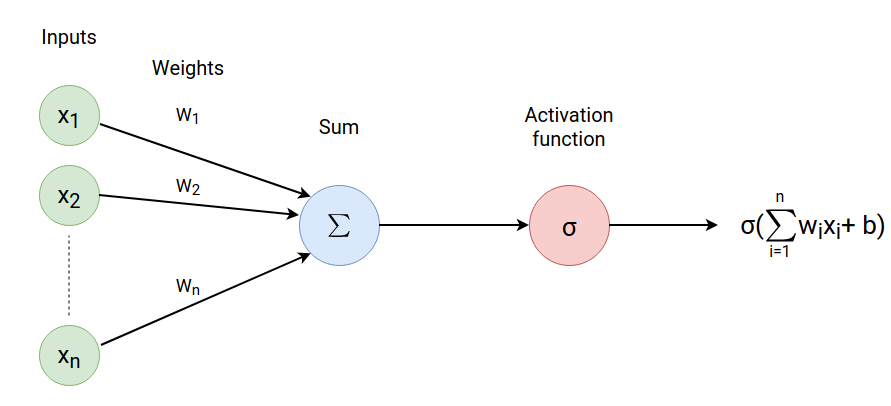
\includegraphics[width=0.9\textwidth]{figures/perceptron.png}
    \caption{\textbf{The Perceptron} is a fundamental component of many modern neural network architectures. We often refer to these as neurons. It has a single hidden-unit which is connected to some inputs $\textbf{x}$. The perceptron computes the dot product of a weight vector $\textbf{w}$ with the input $\textbf{x}$, optionally adds a bias term, then passes the result through a non-linearity. }
\end{figure}


The perceptron can model a function of this form: $\sigma(\sum_i^{n} \mathbf{w_i} x_i +b) = \sigma(\mathbf{w}^\top \textbf{x} + b)$. Often, we select the non-linear function $\sigma$ to be one of the following:

\begin{subequations*}
  \begin{tabularx}{\textwidth}{X{2cm}X{2cm}X}
  \begin{equation*}
     \text{sigmoid} = \frac{1}{1+e^{-x}}
  \end{equation*}
  & &
  \begin{equation*}
     \text{tanh} = \frac{e^{2x}-1}{e^{2x}+1}
  \end{equation*}
    & &
  \begin{equation*}
     \text{ReLU} = \text{max}(0, x)
  \end{equation*}
  \end{tabularx}
\end{subequations*}

\vspace{5mm} %5mm vertical space

Notably, the perceptron is a linear classifier, and as such it famously cannot accurately classify XOR \cite{Minskyetal1969}. More precisely, given two binary variables $x_1$ and $x_2$, the XOR function returns 1 when exactly one of these binary variables is equal to 1, otherwise it returns 0. After selecting a reasonable loss function such as Mean-Squared Error, and minimizing the loss of our model with respect to the weights $w_1$ and $w_2$ and bias $b$ in our perceptron, we obtain a model which incorrectly classifies at least half of the points. It cannot fit the training data! We show the in Figure \ref{fig:XOR} and refer interested readers to the \href{https://www.deeplearningbook.org/contents/mlp.html}{Chapter 6 of the Deep Learning book} for a more detailed analysis \citep{Goodfellow-et-al-2016}.\\

\begin{figure}[H]
    \centering
    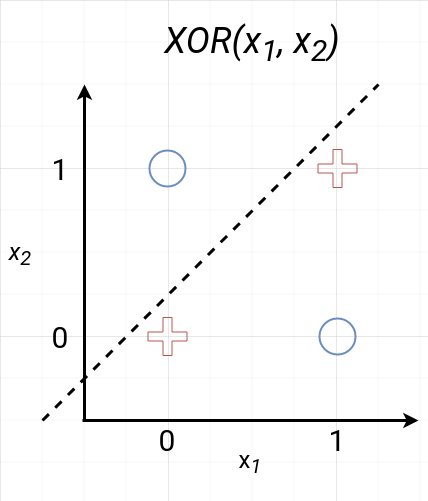
\includegraphics[width=0.35\textwidth]{figures/xor_non_linsep.png}
    \caption{\textbf{The XOR} function is perhaps the simplest non-linear function. Here, we show that the transformation it applies to $x_1$ and $x_2$ cannot be modelled by a perceptron. In other words, we cannot train a perceptron to classify this data because it is not linearly separable and the perceptron is only able to express linear functions.}
    \label{fig:XOR}
\end{figure}

\subsection{The Multi-Layer Perceptron}
The reading in UML \citep{Shalev-Shwartz:2014:UML:2621980} introduces the Multi-Layer Perceptron (MLP) and discusses its expressivity. Here, we will provide a brief and lossy summary. Figure \ref{fig:nn} shows a very small Multi-Layer Perceptron (MLP) which can correctly classify XOR. As you can see, it is composed of 3 perceptrons, 2 in the hidden layer and 1 in the output layer.

\begin{figure}[H]
    \centering
    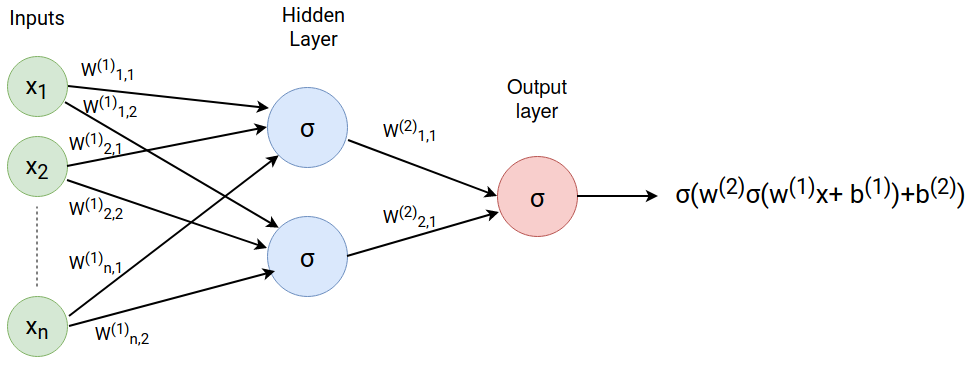
\includegraphics[width=.8\textwidth]{figures/nn.png}
    \caption{\textbf{A Multi-Layer Perceptron} with 2 hidden units and an output layer. This model can learn to classify XOR. }
    \label{fig:nn}
\end{figure}

The MLP is a \textit{feedforward neural network}. Typically, the architecture of a neural network is fixed (i.e., we select the number of neurons, how they are connected, their non-linear activation functions, and their weight initialization) before training. The feedforward network architecture is formalized in \citep{Shalev-Shwartz:2014:UML:2621980} as a directed acyclic graph $G = (V, E)$, with a weight function over the edges, $w: E \to \mathbb{R}$. Nodes on the graph correspond to neurons and $\sigma$ is some non-linearity (e.g., the sign function, threshold function, some sigmoidal function, ReLU).

\vspace{5mm}

The MLP architecture (when the number of units in the hidden layer is permitted to grow) is a \textbf{universal approximator}. In Section \ref{sec:uat} we will discuss the classic result from Cybenko in `89 \citep{cybenko1989approximation} that any neural network with sigmoidal activation (i.e., 1 as $x \to +\infty$ and 0 as $x \to -\infty$ can approximate any continuous function arbitrarily well. While this was the first proof of the universal approximation theorem, many more have followed. Some of these do not rely on this assumption about the non-linearity, in particular Leshno-Lin-Pinkus-Schocken `93 shows the theorem holds iff $\sigma$ is not a polynomial ~\citep{journals/nn/LeshnoLPS93}. Next, we will show a visual proof of the Universal Approximation Theorem.



\section{Universal Approximation Theorem}
\label{sec:uat}

The universal approximation theorem states that any continuous function $f :[0,1]^n \xrightarrow{} [0,1]$
can be approximated arbitrarily well by a Multi-Layer Perceptron with at least 1 hidden layer and a finite number of hidden units.  \par

\subsection{Visual proof of Universal Approximation}
In this section we will present a good intuition for the universal approximation theorem by making a summary of this page \href{http://neuralnetworksanddeeplearning.com/chap4.html}{\underline{http://neuralnetworksanddeeplearning.com/chap4.html}}. (All credit is due to \href{http://neuralnetworksanddeeplearning.com/}{\underline{Michael A. Nielsen}} for all the pictures in this subsection) \\

Say we want to approximate a function with 1 input and 1 output like so:
\begin{figure}[H]
    \centering
    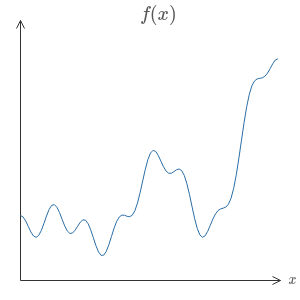
\includegraphics[width=.4\textwidth]{figures/function.png}
    \caption{A continuous function}
\end{figure}

We will first consider a simple MLP with 2 hidden neurons that have a sigmoid activation function, and for now the output neuron will just be linear. \\

\textbf{Step 1} Make a step function with 1 of the neuron.
\begin{figure}[H]
    \centering
    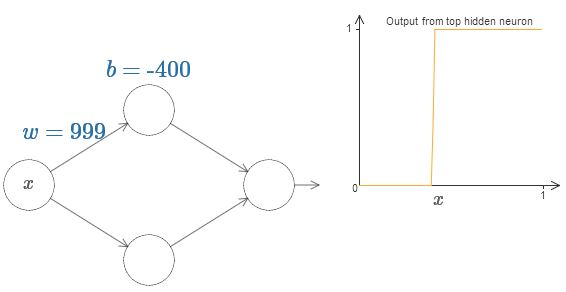
\includegraphics[width=.6\textwidth]{figures/high_weight_function.jpg}
    \caption{For the top neuron, by selecting a large weight, and a bias term as some proportion of that weight, we can construct and position a step function arbitrarily well.}
\end{figure}
Let's focus on the top hidden neuron first, by using a big weight on the top neuron we can approximate the step function with a sigmoid arbitrarily well, and by adjusting the bias we can place it anywhere.
The same argument could be made for the tanh activation, but not for ReLU. In this toy example, we won't be interested in changing the weights of the first layer, they just have to be high enough that we may consider them to be constant. To simplify the plots, we will report only the position of the step, $s$, instead of the weight and bias values. $s$ is easily computed as $s = -\frac{b}{w}$. With these changes, the plot becomes:
\begin{figure}[H]
    \centering
    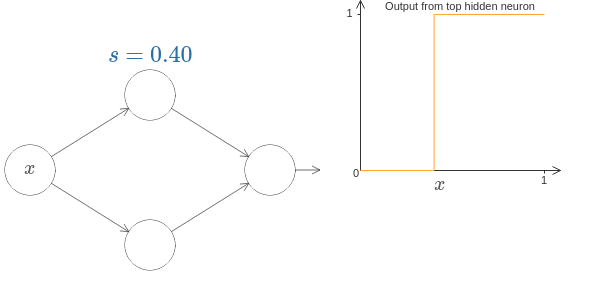
\includegraphics[width=.6\textwidth]{figures/2nn_s.png}
    \caption{Having selected the top neuron's weight to be large, we can re-write the weight and bias of the top neuron as a single variable that describes the position of the step function, $s = -\frac{b}{w}$}
\end{figure}

\textbf{Step 2} We can construct a ``bin'' by setting the bottom neuron to ``step down'' at some later $x$ value.
\begin{figure}[H]
    \centering
    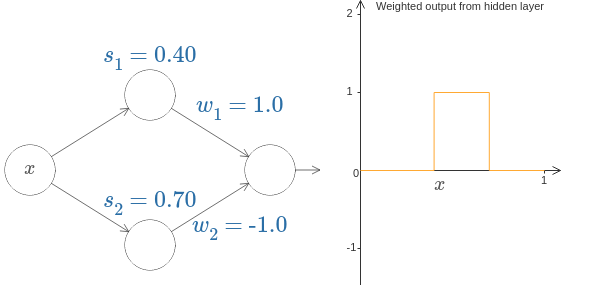
\includegraphics[width=.6\textwidth]{figures/bin.png}
    \caption{Making a bin with 2 opposite step functions}
\end{figure}

As illustrated above, by using the other neuron to make a step function, and setting opposing weights in the second layer, we can effectively approximate a bin and control its position, size and height.
Now you can probably see where this is going, to make things even clearer, we will just use 1 value for both $w_1$ and $-w_2$, called $h$, representing the height of the ``bin".

\begin{figure}[H]
    \centering
    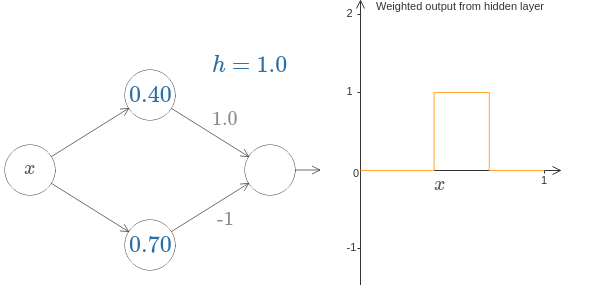
\includegraphics[width=.6\textwidth]{figures/bin_h.png}
    \caption{Making a bin with 2 opposite step functions}
\end{figure}

\textbf{Step 3} In this final step, we show that we can approximate a discretized $f(x)$ by combining several ``bins" to make a histogram approximating the function. Illustrated below is a very rough approximation using only 5 bins (10 hidden units), but we can obviously make it as sharp as we like by adding more bins. Recall that the neuron in the output layer is linear. If we instead added a sigmoid activation function on the output unit we just have to approximate $\sigma^{-1}\circ f$ instead of $f$, which we can do with the same method.


\begin{figure}[H]
    \centering
    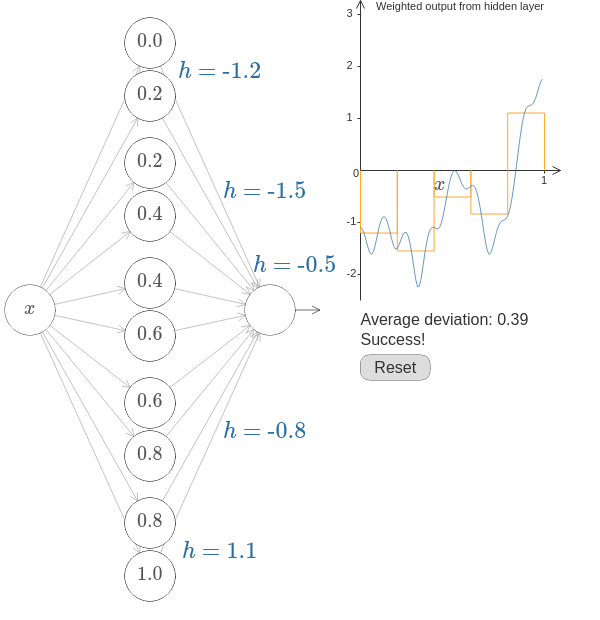
\includegraphics[width=.6\textwidth]{figures/discretize.png}
    \caption{Approximating $f$ with an histogram}
\end{figure}

\textbf{Remarks}: It is important to remember that although an MLP is a universal approximator, that does not mean that it can \textit{learn} any function through gradient descent. Indeed, many important problems are not learnable in practice through gradient descent ~\citep{failures2017shalevshwartz}, even in the context of i.i.d. examples. There are even fewer guarantees on the performance of neural networks when applied to data outside the domain seen during training; this is an active area of research ~\citep{xu2021neural}.

\textit{Exercise for the reader}: if we wanted to use this technique to approximate an \textit{L-Lipschitz} function $f: \mathbb{R} \rightarrow \mathbb{R}$ on the interval $[0, 1]$ with an error at most $\epsilon$ at any point, how many bins would we need?  


\subsection{Cybenko's Universal Approximation Result}
In this subsection we will present Cybenko's \cite{cybenko1989approximation} result for Universal Approximation of MLPs with a single hidden layer and any sigmoidal non-linearity. This was the first result achieved of this kind, and is based on the following intuition. Artificial neural networks are formed by compositions and superpositions of a single, simple nonlinear activation function. The output of the network is the value of the function that results from that particular composition and superposition of non-linearities as activated by the input. First, we define a \textit{sigmoidal function} $\sigma$ as:
$$
\sigma(x) \to
\begin{cases}
1 \text{\quad as } x\to+\infty \\
0 \text{\quad as } x\to-\infty
\end{cases}
$$
\textit{\textbf{N.B.} sigmoidal functions are usually assumed to be monotonic increasing, but this is not necessary for this result.}

\begin{thm}
Let $C([0,1]^n)$ denote the set of all continous function $[0, 1]^n \to \mathbb{R}$, let $\sigma$ be any sigmoidal activation function then the finite sum of the form   
$f(x) = \sum_{i=1}^{N} \alpha_i \sigma(\mathbf{w}_i^\top x + b_i)$ is dense in $C([0,1]^n)$
\end{thm}

Informally, this theorem is saying that for any $g \subset C([0,1]^n)$ and any $\epsilon >0$, there exists $f: x \rightarrow \sum_{i=1}^{N} \alpha_i \sigma(\mathbf{w_i}^\top x +b)$ such that $|f(x)-g(x)|<\epsilon$ for all $x \subset [0,1]^n$. So, for any $\epsilon$ you choose, there is a function in this parametric family that is arbitrarily close to what your desired function. The $\epsilon$ is ``hiding'' in the statement of density.

\begin{figure}[htp]
    \centering
    \[
    \begin{tikzpicture}
      \begin{axis}[ 
        xlabel=$x$,
        ylabel=$y$,
        width=10cm
      ] 
        \addplot[black ] {sin(deg(x))};
        \addplot[red,dashed ] {sin(deg(x))+sin(deg(x*10))*0.2};
         \node[below,black] at (450,0.8) {absolute difference between $f(x)$ and $g(x)$ is $\epsilon$};
        \legend{$f(x)$, $g(x)$}
      \end{axis}
    \end{tikzpicture}
    \]
    \caption{We show the fitting of $f(x)$ to $g(x)$ within a tolerance of $\epsilon$ to illustrate the Cybenko universal approximation theorem.}
    \label{fig:cybenko-approx}
\end{figure}

Cybenko's result relied upon the Kolmogorov-Arnold Representation theorem described in the next section. A similar result was independently obtained by Hornik\cite{hornik1989multilayer} and also by Funahashi\cite{funahashi1989approximate} using different tools. Hornik's proof relies on the Stone-Weierstrass Theorem which states that every continuous function defined on a closed interval $[a, b]$ can be uniformly approximated as closely as desired by a polynomial function.

\subsection{Kolmogorov-Arnold Representation theorem}
The Kolmogorov-Arnold representation theorem (or superposition theorem) \cite{kolmogorov1957representation} states that every multivariate continuous function can be represented as a superposition of continuous functions of one variable.\par
It solved a more general form of Hilbert's thirteenth problem \cite{abhyankar1997hilbert} which was questioning whether a solution to $7^{th}$ degree equations could be expressed by a finite sum of two-variable functions.\par

\begin{thm}
Any continuous function $f :[0,1]^n \xrightarrow{} \mathbb{R}$ can be written as 
$$ f(x) =f(x_1,..,..,x_n) =  \sum_{q=1}^{Z_n = 2n+1} \phi_q\left(\sum_{p=1}^{n} \Psi_pq(x_p)\right) $$
\end{thm}
This implies, among other things, that if we could chose a ``bespoke'' non-linearity for each unit we can represent any continuous function \textbf{exactly} with a NN with 1 hidden layer. In practice we don't care about the $\epsilon$ in the approximation of Cybenko's result, so the Kolmogorov-Arnold Representation theorem is more powerful than we need.


\section{The expressive power of Deep neural networks}
\label{sec:expressive-dnns}
This section contains several results that relate certain classes of problem, neural network architecture choices, and the number of parameters required to achieve an error on the aforementioned problem. 

\subsection{Expressivity of MLPs}
In order to further study the expressivity of the feedforward network, we next discuss which Boolean functions (functions from $\{\pm 1\}^n \to \{\pm 1\}$ can be implemented by $\mathcal{H}_{V, E, \text{sign}}$. The non-linearity selected here is the sign function (1 if input is positive, -1 if input is negative), but the result can also be shown for other non-linearities.

\begin{clm}
$\forall n$, there exists a graph $(V, E)$ of depth 2, s.t. $\mathcal{H}_{V, E, \text{sign}}$ contains all functions from $\{0, 1\}^n \to \{0, 1\}$.
\end{clm}

In order to prove this claim, we will construct a network which can compute any Boolean function. However, this network might be exponentially large, and in fact we will see in Theorem \ref{thm:exponential} that it is impossible to express all Boolean functions using a network of polynomial size.

\begin{proof}
We construct a graph with $|V_0| = n + 1$, $|V_1| = 2^n + 1$, and $|V_2| = 1$. Let $E$ be all possible edges between adjacent layers. Now, let $f: \{\pm 1\}^n \to \{\pm 1\}$ be some Boolean function. We need to show that we can adjust the weights so that the network will implement $f$. Let $\textbf{u}_1, \dots, \textbf{u}_k$ be all the vectors in $\{\pm 1\}^n$ on which $f$ outputs 1. Observe that for every $i$ and every $\textbf{x} \in \{ \pm 1\}^n$, if $\textbf{x} \neq \textbf{u}_i$, then $\langle\textbf{x}, \textbf{u}_i \rangle \leq n - 2$ and if $\textbf{x} = \textbf{u}_i$ then $\langle\textbf{x}, \textbf{u}_i \rangle = n$. 
\vspace{5mm}
It follows that the function $g_i(\textbf{x}) = \text{sign}(\langle\textbf{x}, \textbf{u}_i \rangle - n + 1)$ equals 1 iff $\textbf{x} = \textbf{u}_i$. We can adapt the weights between $V_0$ and $V_1$ so that for every $i \in [k]$, the neuron $v_{1, i}$ implements the function $g_i(\textbf{x})$. Finally, we observe that $f(\textbf{x})$ is the disjunction of the functions $g_i(\textbf{x})$ and can therefore be written as $$f(\textbf{x)} = \text{sign} \bigg(\sum_{i=1}^k g_i(\textbf{x}) + k - 1 \bigg)$$
This procedure defines a way to set the weights of a depth-2 network to compute an arbitrary Boolean function, thereby concluding our proof.
\end{proof}

\begin{thm}[Shallow Networks Require Exponential Parameters to Implement Boolean Functions]
\label{thm:exponential}
For every $n$, let $s(n)$ be the minimal integer such that there exists a graph $(V, E)$ with $|V| = s(n)$ such that the hypothesis class $\mathcal{H}_{V,E,\text{sign}}$ contains all the functions from ${0, 1}^n \to {0, 1}$. Then, $s(n)$ is exponential in $n$. Similar results hold for $\mathcal{H}_{V,E,\sigma}$ where $\sigma$ is the sigmoid function.
\end{thm}

\begin{proof}
Suppose that for some $(V, E)$ we have that $\mathcal{H}_{V, E, \text{sign}}$ contains all functions from $\{0, 1\}^n \to \{0, 1\}$. It follows that it can shatter the set of $m = 2^n$ vectors in $\{0, 1\}^n$ and hence the VC dimension of $\mathcal{H}_{V, E, \text{sign}}$ is $2^n$. On the other hand, the VC dimension of $\mathcal{H}_{V, E, \text{sign}}$ is bounded by $O(|E|log(|E|)) \leq O(|V|^3)$ (shown in Section 20.4 of \citep{Shalev-Shwartz:2014:UML:2621980}). This implies that $|V| \geq \Omega(2^{\frac{n}{3}})$ which concludes our proof for the case of networks with the sign activation function. The proof for the sigmoid case is analogous.
\end{proof}

So, it is impossible to express all Boolean functions of $n$ bits using a depth-2 network of size polynomial in $n$. And it's possible to fit any continuous function arbitrarily well. What about other classes of problem? Or with other constraints on the network? We will see this next.

% It has also been shown that it is impossible for a shallow network to classify n-bit parity in a sub-linear number of weights. Parity is the problem of mapping $n$ binary variables to 0 when an odd number take on the value 1, and to 1 when an even number take on the value 1. In the 2-bit case, this problem reduces to classifying XOR. The N-bit parity task requires N features of the form: are at least m bits on? Each feature must look at all the components of the input. 

\vspace{5mm}


\subsection{A view from the width (Lu et al. 2017)}
In the previous sections, we focused on the setting of depth-bounded (e.g. depth-2) neural networks. With \cite{lu2017expressive} we're going to see some interesting results for \textbf{width-bounded} neural networks instead !

\begin{thm}
(Universal Approximation Theorem for Width-Bounded ReLU Networks).
For any Lebesgue-integrable function $f:\mathbb{R}^n \to \mathbb{R}$ and any $\epsilon > 0$, there exists a fully-connected ReLU network $A$ with width $d_m \leq n + 4$, such that the function $F_A$ represented by this network satisfies
$$\int_{\mathbb{R}^n} |f(x)-F_A(x)|dx < \epsilon$$
\end{thm}
This theorem states that any continuous function $f: \mathbb{R}^n \to \mathbb{R}$ can be approximated by a deep ReLU network with width $\leq n+4$.

\begin{thm}
    Let $n$ be the input dimension. For any integer $k \geq n+4$ there exists $F_{\alpha}: \mathbf{R^n} \rightarrow \mathbf{R}$ represented by a relu neural network $\alpha$ with width $d_m= 2k^2$ and depth $h=3$ such that for any constant $b>0$, there exists an $\epsilon>0$ and for any function $F_{\beta}: \mathbf{R^n} \rightarrow \mathbf{R}$ represented by a ReLu neural network $\beta$ whose parameters are bounded in $[-b,b]$ with width $d_m \leq k^{\frac{3}{2}}$ and depth $h \leq k+2$ the following inequality holds
    $$\int_{\mathbf{R}} |F_{\alpha} - F_{\beta}| dx \geq \epsilon$$
\end{thm}

This theorem states that there are networks such that reducing width requires increasing in the size to compensate, which is similar to that of depth qualitatively.

\subsection{Representation benefits of deep NN (Telgarsky 2015)}
In this section, we want to show interesting results from \cite{telgarsky2015representation}, that will allow us to compare the expressivity of wide networks against deep and recurrent networks, on a specific classification problem. Let n-ap (\textit{n-alternating-points}) be the set of $n := 2^k$ points  uniformly spaced within $[0, 1-2^{-k}]$ with alternating labels. We will use different types of neural network to fit this dataset, and see the number of parameters required to achieve a certain classification error.
\begin{figure}[H]
    \centering
    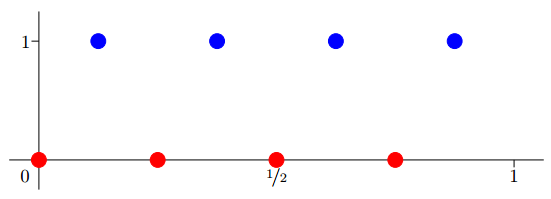
\includegraphics[width=.6\textwidth]{figures/nap.png}
    \caption{The $2^3$-ap \cite{telgarsky2015representation}}
\end{figure}

In the following theorems we will note $\mathscr{N}(\sigma, m, l)$ the set of function given by a feedforward neural network with activation $\sigma$ and $l$ layers with at most $m$ nodes. The ReLU activation will be noted $\sigma_R$ and the classification error $\mathcal{R}_z$.

\begin{thm}
\label{thm:telgarskyffn}
With $m \leq 2^{(k-3)/(l-1)}$, for any positive integer $k$, $\exists$ a collection of $n:=2^k$ points $S = (x_i,y_i)^n_{i=1}$ where $x_i \in [0, 1], y \in \{0, 1\}$ such that \\
$$\min_{f\in\mathscr{N}(\sigma_R, m, l)} \mathcal{R}_z(f) = \frac{1}{6} \quad \quad \text{and} \quad \quad \min_{g\in\mathscr{N}(\sigma_R, 2, 2k)} \mathcal{R}_z(g) = 0$$
\end{thm}

Notably, if we look at the case of 2 layered networks, this tells us that even with $2^{k-3}$ units in the hidden layer, the wide network is going to missclassify $\frac{1}{6}$ of the points, whereas a deep network with $2k$ hidden layers with 2 units each can achieve 0 classification error. What about a recurrent network?  \\

Let $\mathscr{R}(\sigma, m, l, k)$ denote k iterations of a recurrent neural network, every $f \in \mathscr{R}(\sigma, m, l, k)$ can be expressed as some fixed network $g \in \mathscr{N}(\sigma, m, l)$ applied k times:
$$f(x) = g^k(x) = \underbrace{(g\circ g \cdots \circ g)}_\text{k times}(x)$$

Consequently, $\mathscr{R}(\sigma, m, l, k) \subseteq \mathscr{N}(\sigma, mk, l)$ but the former has $\mathcal{O}(ml)$ parameters whereas the latter has $\mathcal{O}(mlk)$ parameters. Lastly we define the following functions:

\begin{defn}[Sawtooth]
A function $f: \reals \xrightarrow{} \reals$ is $t$-sawtooth if it is piece-wise linear with $t$-pieces
\end{defn}
We can say for example that $\sigma_R$ (ReLU) is a 2-sawtooth function, decision stumps used in boosting are also 2-sawtooth, and decision trees with t-1 nodes are t-sawtooth.

\begin{thm}
\label{thm:telgarskyrec}
Let positive integer k, number of layers l, and number of nodes per layer $m$ be given. \\
Given a t-sawtooth $\sigma : \mathbb{R} \to \mathbb{R}$ and $n := 2k$ points as specified by the n-ap, then \\
$$\min_{f\in\mathscr{N}(\sigma, m, l)} \mathcal{R}_z(f) \geq \frac{n-4(tm)^l}{3n} \quad \quad \text{and} \quad \quad \min_{g\in\mathscr{R}(\sigma_R, 2, 2, k)} \mathcal{R}_z(g) = 0$$
\end{thm}
In summary, this means that on the $2^k$-ap, one needs exponentially (in k) many parameters with a wide network, linearly many parameters with a deep network and constantly many parameters with a recurrent network.

\subsubsection{Analysis}
The required reading ~\citep{telgarsky2015representation} provides a proof of the lower bound via a counting argument which tracks the number of times a function within $\mathbb{R}(\sigma;m,l)$ can cross $\frac{1}{2}$. The upper bound is proved via the construction of a network $\mathbb{R}(\sigma_R; 2, 2)$ which can be composed with itself $k$ times to exactly fit the $n$-ap. These bounds together prove Theorems \ref{thm:telgarskyffn} and \ref{thm:telgarskyrec}.\\

While these notes focus on the \textit{parameters} in the network, the parametric requirement of each architecture is itself produced by a more fundamental idea: how adding and composing sawtooth functions grows their complexity. In Lemma 2.3 of ~\citep{telgarsky2015representation}, Telgarsky claims:

\begin{lemma}
Let $f: \mathbb{R} \to \mathbb{R}$ and $g: \mathbb{R} \to \mathbb{R}$ be respectively $k-$ and $l-$sawtooth. Then $f + g$ is $(k + l)-$sawtooth, and $f \circ g$ is kl-sawtooth.
\end{lemma}

This lemma says that the addition of sawtooth functions results in a function which is ``as bumpy as both of the functions together'', while the \textit{composition} of them is multiplicatively as bumpy. This multiplication of non-linear complexity is fundamental to the increased expressive power of deep neural networks. Put another way, depth is exponentially more expressive than width \textbf{because} composition yields more complex functions than summation.




% \subsubsection{Upper bound proof [WIP]}
% \begin{lemma}
% If f is t-sawtooth, g is s-sawtooth, then we have \\
% $f+g$\ \ is (s+t)-sawtooth \quad \quad \quad $f\circ g$\ \ is st-sawtooth
% \end{lemma}
% \begin{lemma}
% If $\sigma$ is t-sawtooth, then every f \in \mathscr{N}($\sigma$;m,l) is $(tm)^l$-sawtooth
% \end{lemma}

% Let us define the "mirror map" $f^k_m: \mathbb{R}\to\mathbb{R}$ as figure shows:
% \begin{figure}[H]
%     \centering
%     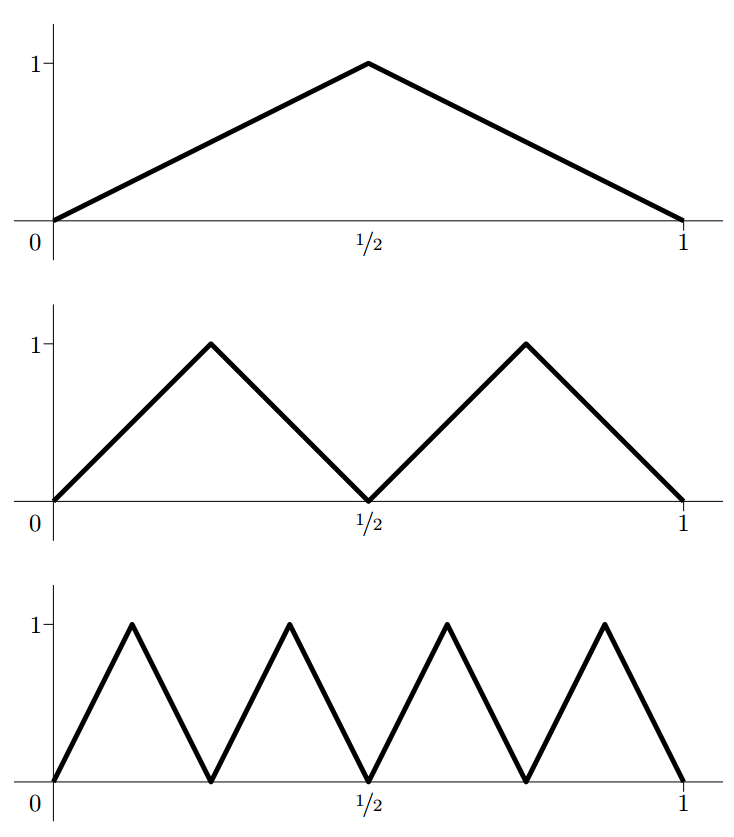
\includegraphics[width=.6\textwidth]{figures/fmk.png}
%     \caption{$f_m$, $f^2_m$ and $f^3_m$ \cite{telgarsky2015representation}}
% \end{figure}

% Note that $f^k_m \in \mathscr{R}(\sigma_R;2,2,k) \subseteq \mathscr{N}(\sigma_R;2,2k)$.

%----------------------------------------https://www.overleaf.com/project/5c6c50cc5b86f10a80c2eff0
% \section*{Acknowledgments} 

%----------------------------------------
\bibliographystyle{abbrvnat}
\bibliography{Refs/lec11}
%----------------------------------------

\end{document}
 